\documentclass[french,a4paper,18pt]{article}
\usepackage{graphicx} % Required for inserting images
\usepackage[style=authoryear, backend=biber]{biblatex}
\usepackage[left=1cm,right=1cm,top=1cm,bottom=2cm]{geometry}
\usepackage{hyperref}
\usepackage{csquotes}
\usepackage{animate}
\usepackage[T1]{fontenc}
\usepackage{amsmath}
\usepackage{multicol} % Package for multi-column layout
\usepackage[french]{babel}
\usepackage{caption} % for \captionof command
\usepackage{adjustbox}
\usepackage{listings}

\title{Apprentissage non-supervisé}
\author{Augustin Bresset | Guillaume Macquart De Terline}
\date{Février 2024}

\begin{document}

\maketitle

\begin{figure}[h]
    \centering
    
\includegraphics[scale=0.2]{../images/logo-tsp-fond-blanc.png}
\end{figure}

\tableofcontents
\twocolumn
% Your content here

\section{Introduction}

L'apprentissage non-supervisé est une branche de l'apprentissage automatique qui consiste à apprendre à partir de données non étiquetées. 
L'objectif est de trouver des structures dans les données, comme des groupes ou des clusters. 
L'apprentissage non-supervisé est souvent utilisé pour explorer des données et pour trouver des modèles cachés. 
Il est également utilisé pour la réduction de dimensionnalité, la visualisation de données et la génération de données.
Dans cet article nous allons étudier et comparer les algorithmes suivants : K-means, K-medoids DBSCAN et Modèle à Mélange de Gaussiennes.

Pour faire ceci, nous allons utiliser le jeu de données MNIST qui est un jeu de données de chiffres manuscrits.
Cela va nous permettre de facilement visualiser les résultats des algorithmes à travers un exemple concret.
On s'attend à ce que les algorithmes trouvent des clusters correspondant à des chiffres similaires. 
Cependant, il est important de noter que les algorithmes ne connaissent pas les étiquettes des chiffres et ne savent pas quels chiffres sont similaires.
C'est pourquoi on s'attend aussi à une confusion entre les chiffres similaires, comme le 3 et le 8 par exemple.

Enfin on va pouvoir comparer les performances des algorithmes en utilisant des métriques comme l'indice de silhouette.

\subsection{Base de données MNIST}
La base de données MNIST est un jeu de données de chiffres manuscrits. 
Chaque chiffre manuscrit est représenté par une image de 28x28 pixels 
Chaque pixel est représenté par un nombre entier entre 0 et 255, qui correspond à la luminosité du pixel.
Il y a 60 000 images dans l'ensemble d'entraînement et 10 000 images dans l'ensemble de test.

\begin{figure}[h!]
    \centering
    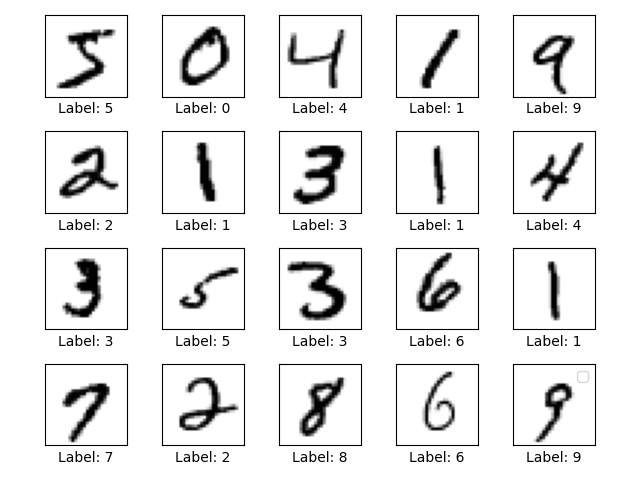
\includegraphics[scale=0.5]{../images/mnist_plot.png}
    \caption{Exemple de chiffres de la base de données MNIST}\label{fig:mnist}
\end{figure}

Ce jeu de données est souvent utilisé pour tester des algorithmes de classification et de clustering.
On peut déjà remarqué ici la grande diversité des écritures des chiffres, ce qui rendra la tâche de clustering difficile.

\subsection{Présentation des modèles}
Pour montrer leur fonctionnement, on génère un jeu de données synthétique avec 300 points regroupés dans 5 clusters avec une variance de 0.8.
\begin{figure}[h]
    \centering
    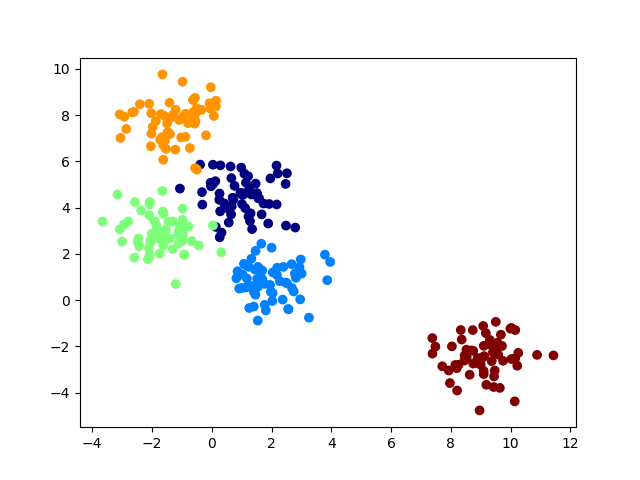
\includegraphics[scale=0.5]{../images/short_simulation_generate_data.png}
    \caption{Data généré de manière synthétique}\label{fig:short_simulation_data}
\end{figure}

On viendra dans la suite chercher à trouver 4 clusters dans ces données.

\subsubsection{K-means}

L'algorithme K-means est un algorithme de clustering qui cherche à partitionner les données en K clusters.
L'algorithme fonctionne de la manière suivante :
\begin{enumerate}
    \item Choisir K points aléatoires dans les données, qui serviront de centres de clusters.
    \item Assigner chaque point de données au centre de cluster le plus proche.
    \item Mettre à jour les centres de clusters en prenant la moyenne des points assignés à chaque cluster.
    \item Répéter les étapes 2 et 3 jusqu'à ce que les centres de clusters ne changent plus.
\end{enumerate}


On obtient les résultats suivants :
\begin{figure}[h]
    \centering
    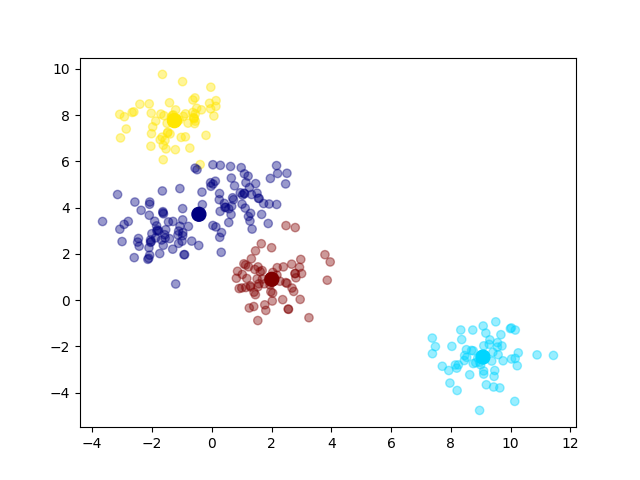
\includegraphics[scale=0.5]{../images/short_simulation_kmeans.png}
    \caption{Résultat de l'algorithme K-means}\label{fig:short_simulation_kmeans}
\end{figure}

On remarque la fusion des deux clusters les plus proches ce qui est cohérent 
étant données que l'on cherche 4 clusters dans un ensemble de données regroupés en 5 clusters.
On verra que cette remarque s'appliquera à tous les algorithmes.

\paragraph{Fonction de coût}
La fonction de coût utilisée par l'algorithme prend en compte la distance entre les points et les centres des clusters.
Elle est aussi appelée "inertie" et est définie comme suit :
\begin{equation}
    J = \sum_{i=1}^{n} \sum_{k=1}^{K} 1\{c_{i} = k\} ||x_{i} - \mu_k||^2
    \label{eq:kmeans_cost}
\end{equation}

Avec :
\begin{itemize}
    \item $n$ le nombre de points de données
    \item $K$ le nombre de clusters
    \item $c_{i}$ le cluster auquel le point de données $x_{i}$ est assigné
\end{itemize}
\subsubsection{K-medoids}

L'algorithme K-medoids est une variante de l'algorithme K-means. 
La différence principale est que K-medoids utilise des points de données comme centres de clusters, alors que K-means utilise des moyennes.
Cela rend K-medoids plus robuste aux valeurs aberrantes que K-means.
L'algorithme fonctionne de la manière suivante :
\begin{enumerate}
    \item Choisir K points aléatoires dans les données, qui serviront de centres de clusters.
    \item Assigner chaque point de données au centre de cluster le plus proche.
    \item Mettre à jour les centres de clusters en prenant le point de données qui minimise la somme des distances aux autres points assignés à chaque cluster.
    \item Répéter les étapes 2 et 3 jusqu'à ce que les centres de clusters ne changent plus.
\end{enumerate}

On a aussi appliquer cet algorithme sur le jeu de données précédent.
\begin{figure}[h!]
    \centering
    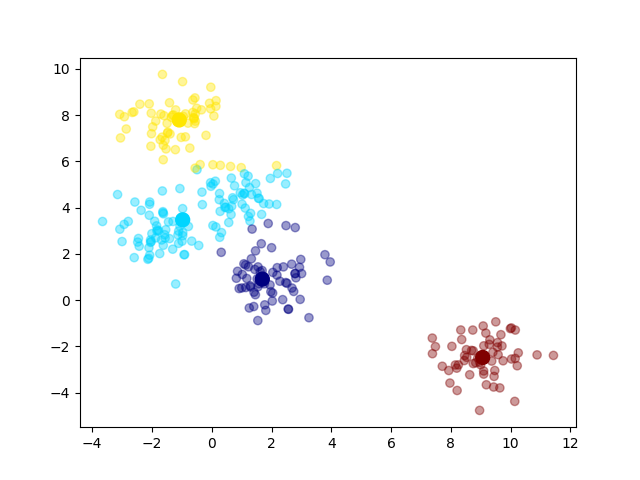
\includegraphics[scale=0.5]{../images/short_simulation_kmedoids.png}
    \caption{Résultat de l'algorithme K-medoids}\label{fig:short_simulation_kmedoids}
\end{figure}

\subsubsection{Modèle à Mélange de Gaussiennes}

Un modèle de mélange gaussien (GMM) est un modèle probabiliste qui cherche à modéliser les données comme un mélange de distributions gaussiennes.
L'algorithme fonctionne de la manière suivante :
\begin{enumerate}
    \item Choisir K points aléatoires dans les données, qui serviront de centres de clusters.
    \item Assigner chaque point de données à une distribution gaussienne en utilisant la loi de Bayes.
    \item Mettre à jour les centres de clusters et les paramètres des distributions gaussiennes en maximisant la vraisemblance des données.
    \item Répéter les étapes 2 et 3 jusqu'à ce que les centres de clusters ne changent plus.
\end{enumerate}

Résultat de l'algorithme sur le jeu de données précédent.
\begin{figure}[h!]
    \centering
    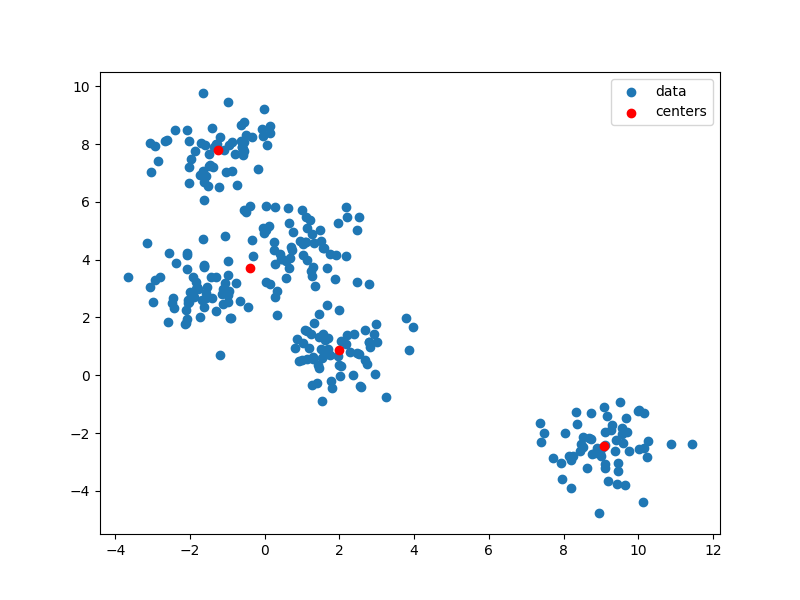
\includegraphics[scale=0.3]{../images/short_simulation_gmm.png}
    \caption{Résultat de l'algorithme Modèle à Mélange de Gaussiennes}\label{fig:short_simulation_gmm}
\end{figure}

\subsubsection{DBSCAN}

DBSCAN est un algorithme de clustering qui est basé sur la densité des points. 
L'algorithme fonctionne de la manière suivante :
\begin{enumerate}
    \item Choisir un point de données aléatoire.
    \item Trouver tous les points de données qui sont à une distance inférieure à un seuil $\epsilon$ du point de données.
    \item Si le nombre de points de données trouvés est supérieur à un seuil $minPts$, alors on crée un cluster avec ces points de données et on recommence à l'étape 1 avec un autre point de données.
    \item Si le nombre de points de données trouvés est inférieur à $minPts$, alors on marque le point de données comme un point de bruit et on recommence à l'étape 1 avec un autre point de données.
\end{enumerate}

On a appliqué cet algorithme sur le jeu de données précédent avec une valeur de $\epsilon$ de 0.2 et une valeur de $minPts$ de 5.
Résultat de l'algorithme sur le jeu de données précédent.
\begin{figure}[h!]
    \centering
    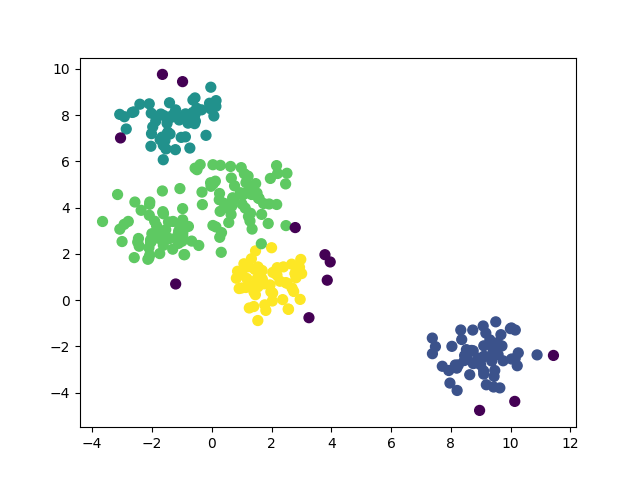
\includegraphics[scale=0.5]{../images/short_simulation_dbscan.png}
    \caption{Résultat de l'algorithme DBSCAN}\label{fig:short_simulation_dbscan}
\end{figure}

On remarque ici que certains points ne sont pas assignés à un cluster, ce sont les points de bruit.

\pagebreak
\section{Étude de K-Means sur la base de données MNIST}


Afin de baisser le temps de calcul, on ne va étudier que les 10 000 premières images de la base de données MNIST.
On aura donc 10 clusters contenant chacun : 
\begin{itemize}
    \item label 0 : 1001 images
    \item label 1 : 1127 images
    \item label 2 : 991 images
    \item label 3 : 1032 images
    \item label 4 : 980 images
    \item label 5 : 863 images
    \item label 6 : 1014 images
    \item label 7 : 1070 images
    \item label 8 : 944 images
    \item label 9 : 978 images
\end{itemize}

\subsection{Étude pour 10 clusters}

On clusterise les images en utilisant les pixels comme features et on recherche 10 clusters.
Cela nous permet d'avoir une première visualisation des résultats de l'algorithme pour un nombre 
de cluster cohérent avec le problème à résoudre.

\begin{figure}[h!]
    \centering
    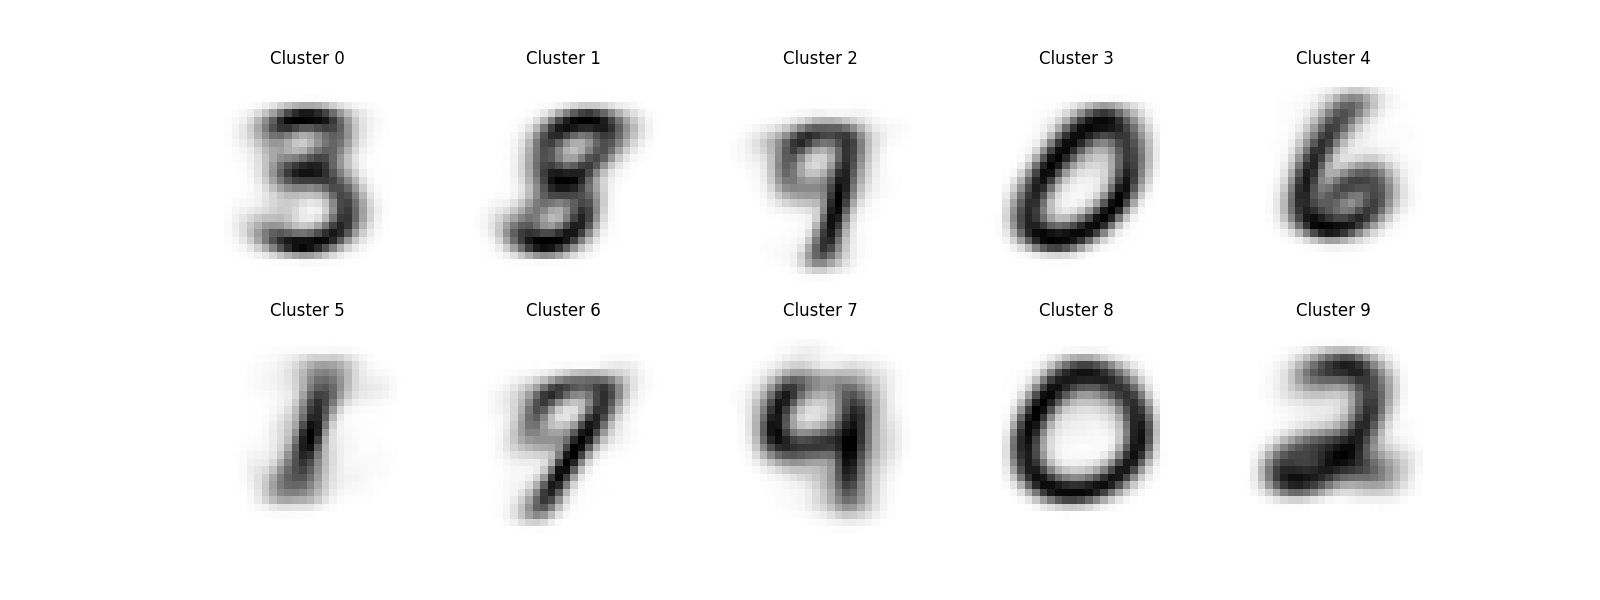
\includegraphics[scale=0.25]{../images/mnist_kmeans_ten_clusters.png}
    \caption{Résultat de l'algorithme K-means sur la base de données MNIST}\label{fig:mnist_kmeans}
\end{figure}

On remarque ici que malgré la présence de 10 clusters, on ne retrouve pas les 10 chiffres.
En effet, deux clusters semblent décrirent le chiffre 0 et trois autres sont flous quant à leur description des chiffres 4 et 9.
Enfin les clusters sont très hétérogènes, ce qui est cohérent avec la diversité des écritures des chiffres.

\subsection{Étude des performances en fonction du nombre clusters : méthode usuelle}

\subsubsection{Fonction de coût}
On peut étudier la fonction de coût[\ref{eq:kmeans_cost}] par rapport au nombre de clusters.
Ici on a tracé la fonction de coût pour un nombre de clusters allant de 2 à 20.

\begin{figure}[h!]
    \centering
    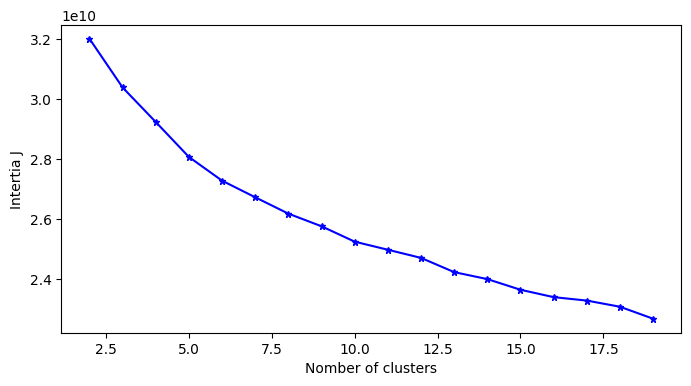
\includegraphics[scale=0.4]{../images/mnist_kmeans_inertia.png}
    \caption{Fonction de coût en fonction du nombre de clusters}\label{fig:mnist_kmeans_cost}
\end{figure}

Il est totalement cohérent que la fonction soit décroissante en fonction du nombre de clusters.
En effet, plus on a de clusters, plus on peut réduire la distance entre les points et les centres des clusters.

\textbf{La méthode du coude} consiste à choisir le nombre de clusters qui correspond à l'endroit où la fonction de coût commence à décroître plus lentement.
Ce choix permet de déterminer le nombre optimal de clusters.

Dans ce cas, la courbe ne présente pas de coude net. Elle ne permet donc pas de déterminer clairement le nombre de clusters optimal.

\paragraph{Indice de silhouette}

L'indice de silhouette est une mesure de la qualité des clusters.
Il est défini comme suit :
\begin{equation}
    s(i) = \frac{b(i) - a(i)}{max(a(i), b(i))}
    \label{eq:silhouette_i}
\end{equation}

Avec :
\begin{itemize}
    \item $a(i)$ la distance moyenne entre le point $i$ et les autres points du même cluster
    \item $b(i)$ la distance moyenne entre le point $i$ et les points du cluster le plus proche
    \item $s(i)$ l'indice de silhouette du point $i$
\end{itemize}

On peut caluler la moyenne groupée par cluster de l'indice de silhouette pour chaque nombre de clusters.
Cela nous permet d'estimer l'homogénéité et la séparation des clusters.

On a tracé la moyenne de l'indice de silhouette pour un nombre de clusters allant de 2 à 12.

\begin{figure}[h!]
    \centering
    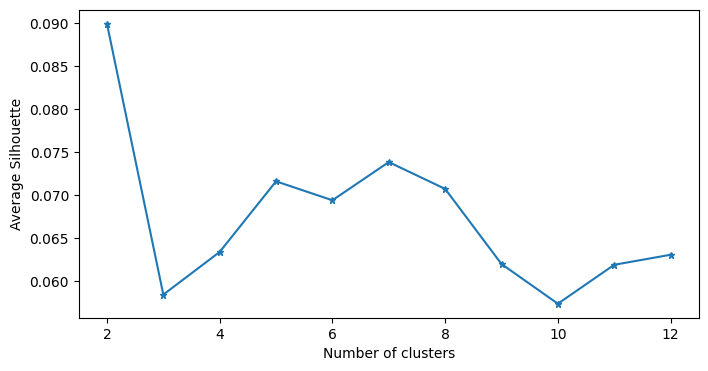
\includegraphics[scale=0.4]{../images/mnist_kmeans_silhouette.png}
    \caption{Indice de silhouette en fonction du nombre de clusters}\label{fig:mnist_kmeans_silhouette}
\end{figure}

On remarque que l'indice de silhouette est maximal pour 2 clusters. 
Cependant on ne va pas prendre cette mesure en compte car en séparant simplement l'espace en deux, 
elle n'est pas représentative de la qualité des clusters. 
On va donc plutôt regarder le nombre suivant de clusters pour lequel l'indice de silhouette est maximal. 
Dans ce cas, le \textbf{nombre de cluster optimal est 7}.

\subsection{Étude des performances en fonction du nombre clusters : méthode alternative}

On viendra faire cette étude en prenant 7 cluster pour les raisons évoquées précédemment.

\subsubsection{Matrice de confusion} 
On peut aussi étudier la matrice de confusion pour chaque nombre de clusters.
Celle ci représente pour la ligne $i$ et la colonne $j$, le nombre de point de label $i$ qui sont dans le cluster $j$.

Pour le choix de 7 clusters, on obtient une matrice de taille 10x7.

\[
\begin{bmatrix}
    812 & 14 & 1 & 4 & 61 & 71 & 38 \\
    0 & 2 & 3 & 1109 & 4 & 9 & 0 \\
    9 & 27 & 6 & 213 & 60 & 627 & 49 \\
    6 & 29 & 19 & 89 & 736 & 142 & 11 \\
    1 & 524 & 366 & 63 & 0 & 5 & 21 \\
    13 & 63 & 124 & 236 & 368 & 33 & 26 \\
    16 & 24 & 0 & 114 & 6 & 15 & 839 \\
    1 & 325 & 646 & 91 & 1 & 5 & 1 \\
    3 & 25 & 68 & 172 & 333 & 326 & 17 \\
    5 & 437 & 477 & 38 & 17 & 2 & 2 \\
    \end{bmatrix}
\]    
\captionof{table}{Matrice de confusion pour 7 clusters}


\subsubsection{Analyse par colonne} 

Chaque colonne représente un cluster.

Une colonne possèdant des valeurs hétérogènes est un bon cluster car il permet de distinguer les différents labels.
On remarque par exemple que la première colonne est très hétérogène, le chiffre 0 est bien représenté avec 812 itérations
alors que le nombre de points des autres labels ne dépasse 16.

On va donc venir étudier la variance de chaque colonne. 
Cependant, on doit normaliser les valeurs pour que la variance soit comparable entre les colonnes.
On étudie la variance normalisée par colonne car une variance élevée correspond à un cluster hétérogène et donc performant.

\[
\begin{bmatrix}
    0.93 & 0.01 & 0.02 & 0.04 & 0.00 & 0.01 & 0.04 \\
    0.00 & 0.00 & 0.00 & 0.00 & 0.54 & 0.00 & 0.00 \\
    0.01 & 0.01 & 0.82 & 0.04 & 0.09 & 0.00 & 0.03 \\
    0.01 & 0.03 & 0.06 & 0.45 & 0.04 & 0.02 & 0.01 \\
    0.00 & 0.34 & 0.01 & 0.00 & 0.03 & 0.19 & 0.02 \\
    0.02 & 0.04 & 0.00 & 0.21 & 0.10 & 0.09 & 0.03 \\
    0.02 & 0.01 & 0.01 & 0.00 & 0.05 & 0.00 & 0.84 \\
    0.00 & 0.24 & 0.01 & 0.00 & 0.04 & 0.32 & 0.00 \\
    0.01 & 0.02 & 0.05 & 0.25 & 0.10 & 0.11 & 0.02 \\
    0.01 & 0.29 & 0.00 & 0.01 & 0.01 & 0.25 & 0.00 \\
\end{bmatrix}
\]
\captionof{table}{Matrice de confusion normalisée par colonne}

\[
\begin{pmatrix}
    0.078 & 0.016 & 0.058 & 0.021 & 0.022 & 0.012 & 0.061
\end{pmatrix}
\]
\captionof{table}{Variance de chaque colonne normalisée}

On remarque une variance élevée pour la première colonne, ce qui est cohérent avec l'analyse précédente.
De même pour la dernière colonne.
À l'inverse la deuxième colonne possède une variance très faible, ce qui est cohérent en raison 
de son homogénéité.

Cependant on remarque que pour la troisième colonne, la variance est comparable avec celle du dernier cluster
alors que l'analyse de la matrice de confusion nous montre que ce cluster est bien moins hétérogène et donc de plus faible qualité.

L'analyse par la variance normalisée n'est donc pas suffisante pour déterminer la qualité des clusters mais 
elle en donne une idée.

\paragraph{Analyse par ligne} 
Chaque ligne représente un label.

De la même manière, on cherche une répartition hétérogène des valeurs pour chaque ligne
afin d'assurer une bonne représentation de chaque label.

On peut procéder de la même manière que pour l'analyse par colonne. 
Ceci nous conduirait à remarquer que les labels 0 et 1 sont bien identifiés
par les clusters 0 et 3.
Tandis qu'il y une confusion dans l'identification des labels 4 et 9 par les différents clusters.

\paragraph{Analyse des labels majoritaires par cluster} 

On peut aussi étudier les labels majoritaires pour chaque cluster 
et les comparer à la présence de ces labels dans les autres clusters.

Ainsi le 0 est bien identifié par le cluster 0 car il est largement majoritaire celui ci 
et les autres clusters le contiennent peu.

Néanmoins, le 4 est majoritaire dans le cluster 1 mais il est aussi très présent dans le cluster 2,
deux clusters qui ne sont pas très hétérogènes.
On peut donc en déduire que le 4 est mal identifié par ces clusters.

\subsubsection{Attribution de Labels Dominants aux Clusters}

On a associé l'étiquette la plus probable à chaque cluster dans le modèle KMeans.
On a ensuite comparé ces étiquettes avec les étiquettes réelles des données pour chaque cluster.

\begin{figure}[h!]
    \centering
    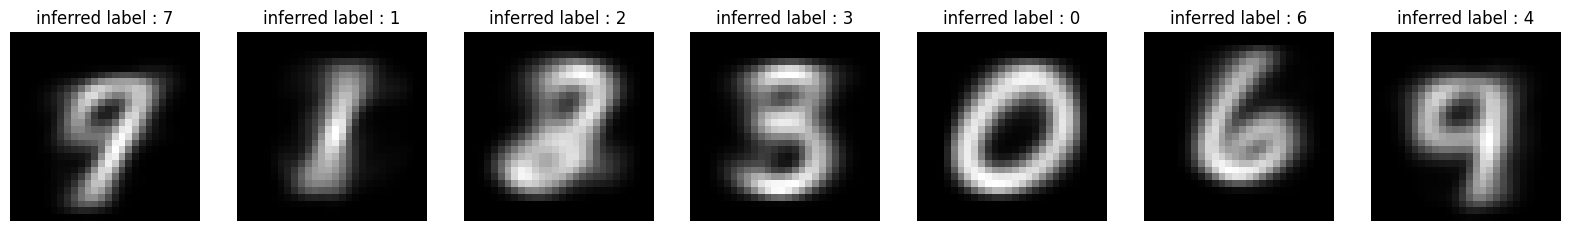
\includegraphics[scale=0.2]{../images/mnist_kmeans_inferred_labels.png}
    \caption{Attribution de Labels Dominants aux Clusters}\label{fig:mnist_kmeans_labels}
\end{figure}

On remarque une confusion entre les chiffres 7 et 9 ainsi qu'entre 4 et 9.
Sinon les clusters semblent bien représenter les chiffres.

\subsubsection{Étude par métrique d'entropie}

On a calculé l'entropie pour chaque cluster vu à la figure \ref{fig:mnist_kmeans_labels}.

\[
\begin{pmatrix}
    7.43838353 & 7.66575343 & 7.12447826 & 7.36581284 & 6.77193556 & 6.90775528 & 7.29301768
\end{pmatrix}
\]
\captionof{table}{Entropie par cluster}

On obtient une moyenne d'entropie de 7.224.

Une entropie faible indique que les points dans le cluster sont relativement bien concentrés autour d'un certain centre.

Ainsi les clusters 4 et 5 possèdent une entropie faible, la disparité des points dans ces clusters est faible
et en effet on remarque sur la figure \ref{fig:mnist_kmeans_labels} que les chiffres sont bien identifiés par ces clusters. 

\begin{figure}[h!]
    \centering
    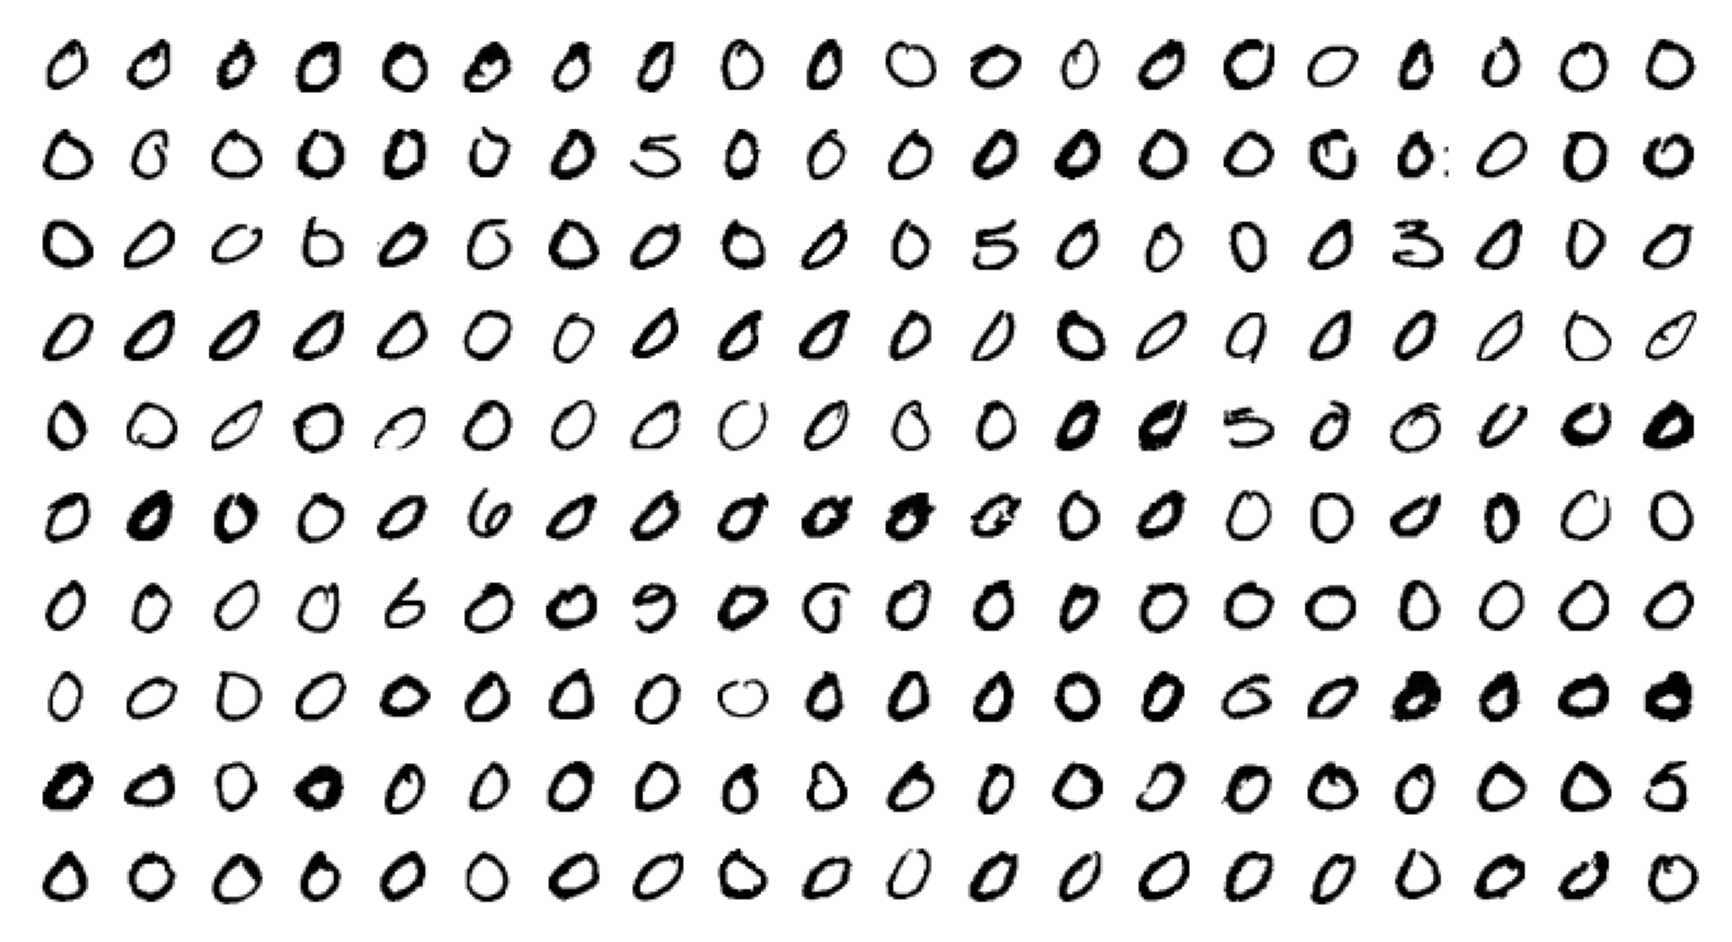
\includegraphics[scale=0.3]{../images/mnist_kmeans_low_entropy_cluster.png}
    \caption{Entropie par cluster}\label{fig:mnist_kmeans_entropy}
\end{figure}


Une entropie élevée indique que les points dans le cluster sont répartis de manière plus éparse ou désordonnée.
On remarque une entropie très élevée pour les clusters 0 et 6, un résultat cohérent 
avec l'analyse de l'attribution des labels dominants dans laquel on remarquer une confusion entre les chiffres 4, 7 et 9.

\begin{figure}[h!]
    \centering
    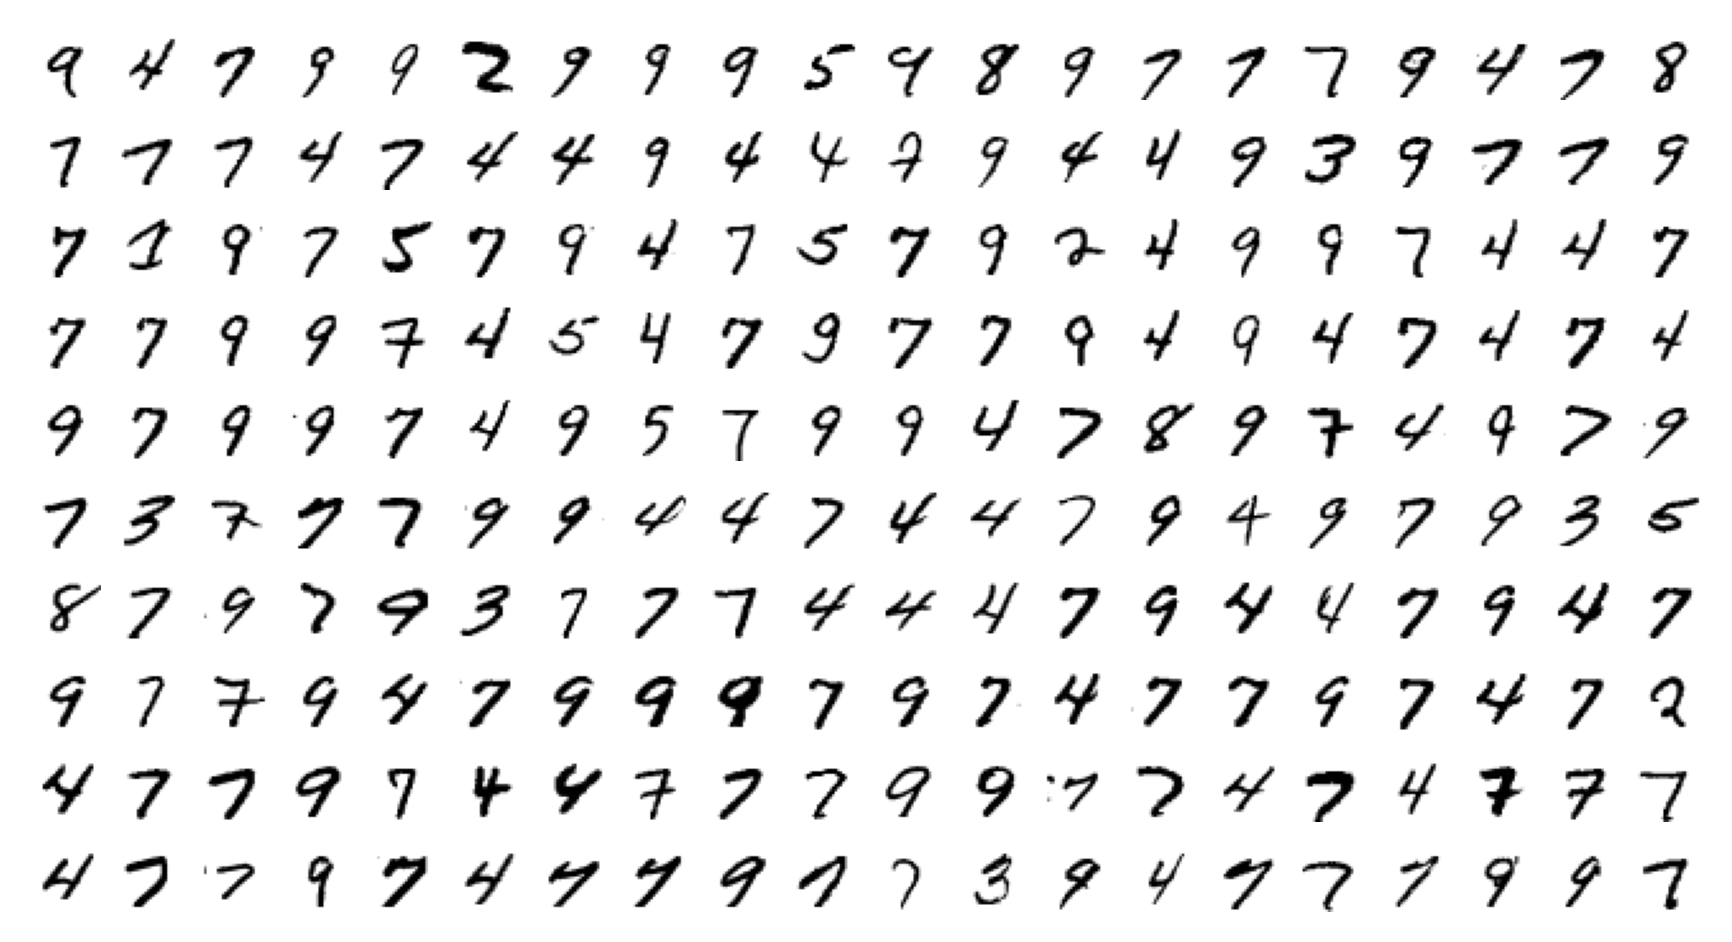
\includegraphics[scale=0.3]{../images/mnist_kmeans_confusion_high_entropy_cluster.png}
    \caption{Entropie par cluster}\label{fig:mnist_kmeans_entropy}
\end{figure}

Le cluster 1 possède l'entropie la plus élevée tout en ayant une attribution de label dominant cohérente.
Cela doit être dû à la présence d'une barre centrale dans la plupart des chiffres ce qui explique 
son entropie élevée mais étant assez distinct des autres chiffres, il est bien identifié par le cluster 1.

\begin{figure}[h!]
    \centering
    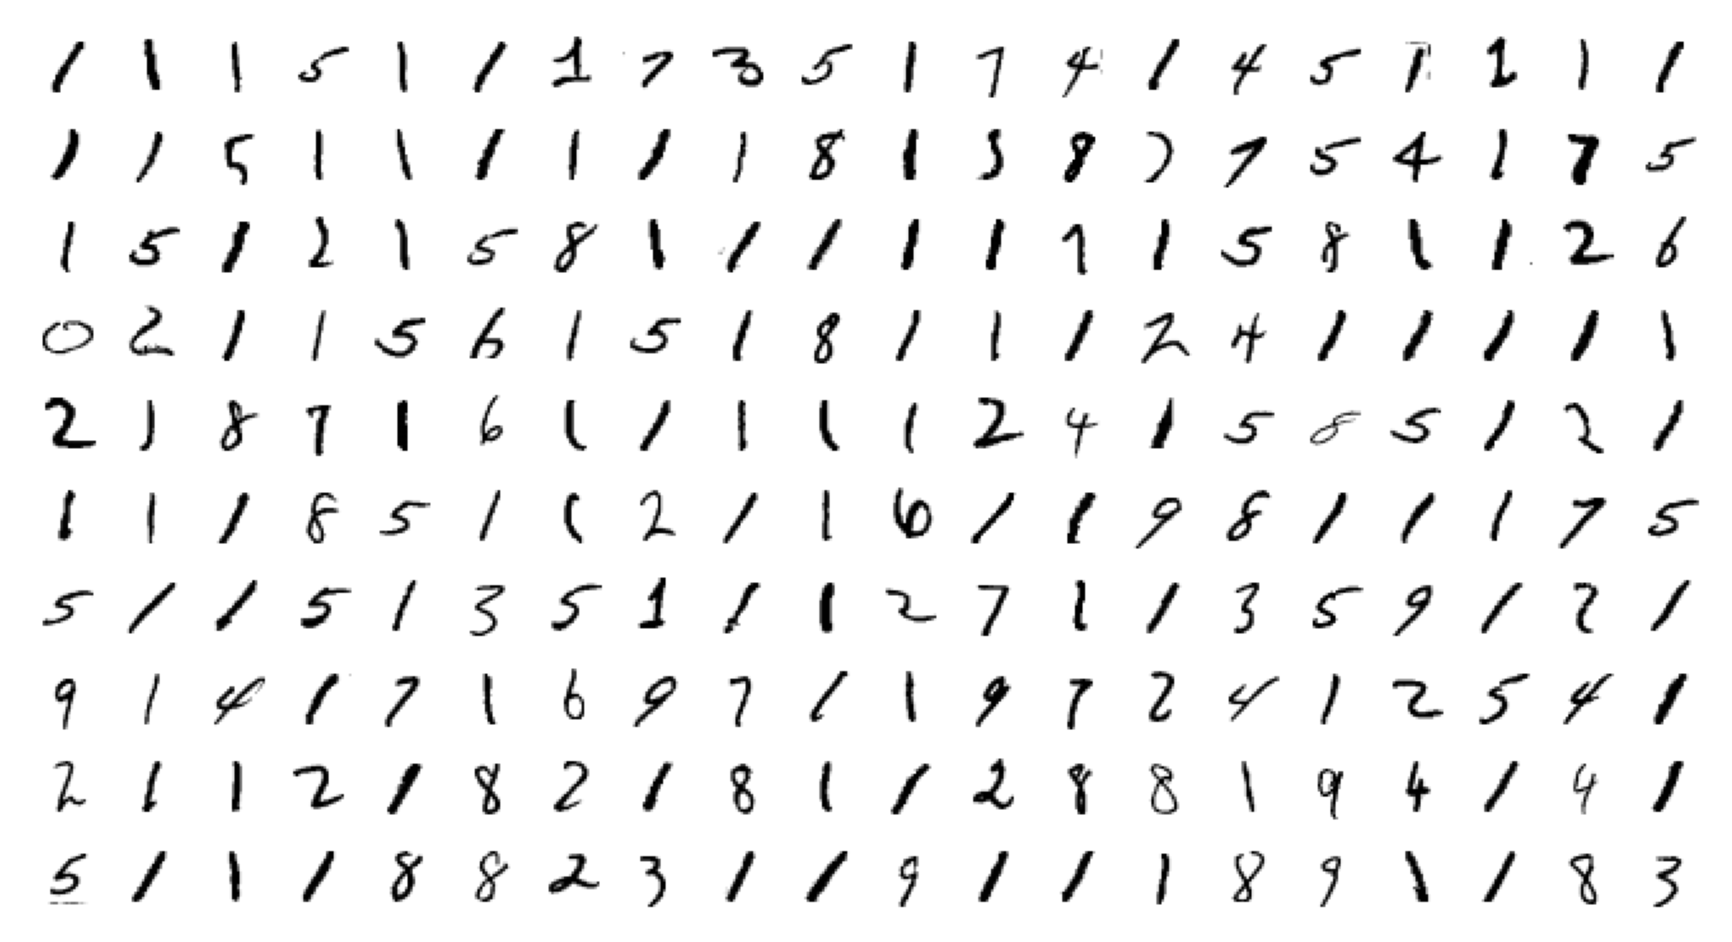
\includegraphics[scale=0.3]{../images/mnist_kmeans_high_entropy_cluster.png}
    \caption{Entropie par cluster}\label{fig:mnist_kmeans_entropy}
\end{figure}

\subsubsection{Exploitation des outils pour l'analyse du nombre de clusters}

On a calculé le taux de bon fonctionnement de l'algorithme KMeans pour un nombre de clusters allant de 2 à 15.

\begin{figure}[h!]
    \centering
    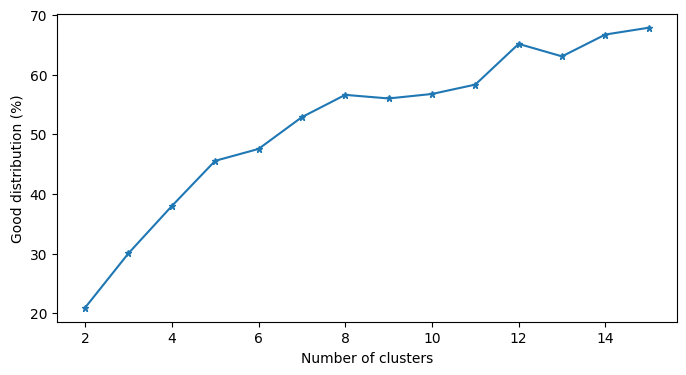
\includegraphics[scale=0.4]{../images/mnist_kmeans_good_distribution.png}
    \caption{Taux de bon fonctionnement de l'algorithme KMeans}\label{fig:mnist_kmeans_score}
\end{figure}
On remarque que le taux de bon fonctionnement en fonction du nombre de cluster est croissant.

\subsection{Comparaison des résultats de méthode alternative avec un nombre différent de clusters}

On va maintenant comparer les résultats obtenus avec 8, 10 et 12 clusters.
On initilisera au même point de départ pour chaque nombre de clusters afin de mieux comparer les résultats.

\subsubsection{Matrice de confusion}
On va venir s'intéresser à la matrice de confusion pour chaque nombre de clusters. 

\begin{figure}[h!]
    \centering
    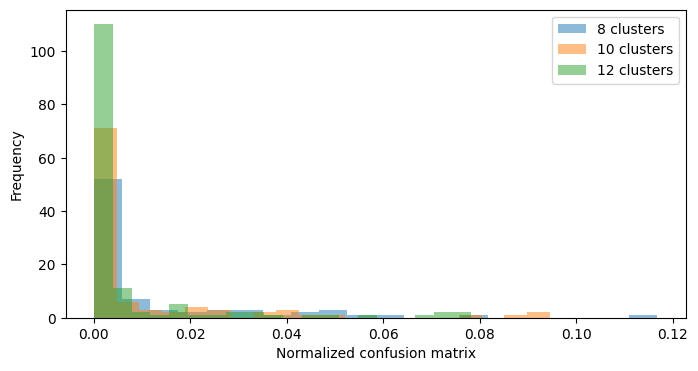
\includegraphics[scale=0.5]{../images/mnist_kmeans_normalized_confusion_matrix_comparaison.png}
    \caption{Matrice de confusion pour 8 clusters}\label{fig:mnist_kmeans_confusion_comparaison}
\end{figure}

On remarque une nette augmentation de la fréquence d'éléments des matrices ayant peu d'iterations.
Cela est un signe de qualité des clusters car on veut que les valeurs soient très hétérogènes 
et concentré sur les extremums.
Á travers les vecteurs de variances normalisées par colonne, on pourra comparer la qualité des clusters.

On a obtenus une moyenne de variance normalisée par colonne de \textbf{0.0274} pour 8 clusters, \textbf{0.0379} pour 10 clusters et \textbf{0.0371} pour 12 clusters.

On remarque une augmentation de la variance normalisée avec l'augmentation du nombre de clusters.

\subsubsection{Analyse par métrique d'entropie}

On a calculé l'entropie pour chaque cluster pour chaque nombre de clusters.


\begin{table}[htbp]
    \centering
    \label{tab:entropies}
    \small % Utilisation d'une taille de police plus petite
    \adjustbox{max width=0.5\textwidth}{
    \begin{tabular}{|c|c|c|c|}
    \hline
    $k$ & Entropies & Moyenne & Variance \\
    \hline
    8 & $6.783 \quad 7.054 \quad 7.120 \quad 6.906 \quad 7.204 \quad 7.519 \quad 6.869 \quad 7.363$ & 7.102 & 0.056 \\
    \hline
    10 & $6.713 \quad 6.946 \quad 7.088 \quad 6.854 \quad 6.593 \quad 7.039 \quad 7.195 \quad 6.592 \quad 6.784 \quad 7.070$ & 6.887 & 0.041 \\
    \hline
    12 & $6.284 \quad 6.873 \quad 7.076 \quad 6.819 \quad 6.560 \quad 6.818 \quad 6.698 \quad 6.553 \quad 6.693 \quad 7.041 \quad 6.777 \quad 6.091$ & 6.690 & 0.075 \\
    \hline
    \end{tabular}
    }
    \caption{Entropies pour différentes valeurs de $k$}
\end{table}

On remarque une baisse de l'entropie moyenne avec l'augmentation du nombre de clusters.
Par nature de l'entropie, ce résultat est cohérent.

\subsection{Conclusion}

On a pu étudier les performances de l'algorithme KMeans sur la base de données MNIST à travers
différentes métriques: la matrice de confusion, la variance normalisée par colonne, l'entropie et le taux de bon fonctionnement.
Ces métriques ont permis de noter les performances de l'algorithme pour différents nombres de clusters.
Et on a pu comparer ces métriques pour un nombre de cluster différent.

Enfin on remarque que l'entrainement de l'algorithme KMeans sur la base de données MNIST n'est pas très performant.
En effet, les clusters obtenus ne sont pas très hétérogènes et ne permettent pas de bien distinguer les différents chiffres
car la distinction n'est pas claire.


\section{Étude de K-medoids sur la base de données MNIST}

On répète la même étude pour l'algorithme K-medoids. Nous travaillons, de même que pour l'algorithme K-means, 
sur les 10 000 premières images de la base de données MNIST.

On clusterise les images en utilisant les pixels comme features et on recherche 10 clusters.
Cela nous permet d'avoir une première visualisation des résultats de l'algorithme pour un nombre 
de cluster à priori cohérent avec le problème à résoudre.

\begin{figure}[h!]
    \centering
    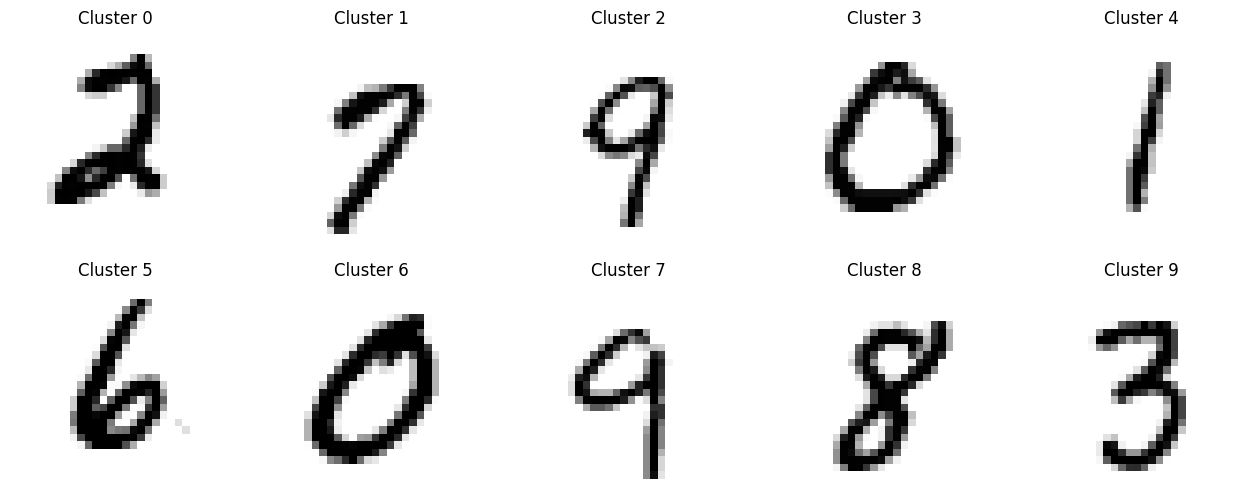
\includegraphics[scale=0.25]{../images/mnist_kmedoids_ten_clusters.png}
    \caption{Résultat de l'algorithme K-medoids sur la base de données MNIST}\label{fig:mnist_kmedoids}
\end{figure}

On remarque ici que malgré la présence de 10 clusters, on ne retrouve pas les 10 chiffres.
En effet, deux clusters semblent décrirent le chiffre 9, ainsi que deux autres le chiffre 0.
On ne retrouve pas les chiffres 4 et 5.

\subsection{Étude des performances en fonction du nombre clusters : méthode usuelle}

\paragraph{Méthode du coude}

Ici on a tracé l'inertie J pour un nombre de clusters allant de 2 à 20. De nouveau, il est cohérent que la fonction Inertie J 
soit décroissante en fonction du nombre de clusters. En effet, plus on a de clusters, plus on peut réduire la distance 
entre les points et les médoïdes, et ainsi faire diminuer la valeur de la fonction de coût, lorsqu'on augmente le nombre de clusters. 

\begin{figure}[h!]
    \centering
    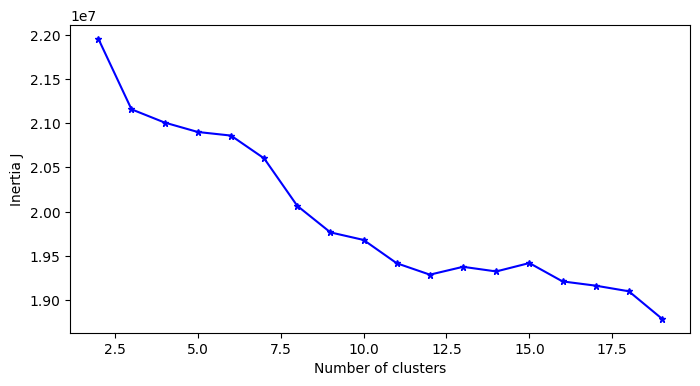
\includegraphics[scale=0.4]{../images/mnist_kmedoids_inertia.png}
    \caption{Fonction de coût en fonction du nombre de clusters}\label{fig:mnist_kmedoids_cost}
\end{figure}

Cependant, comme dans le cas de K-means, la courbe ne présente pas de coude net.
Elle ne permet donc pas de déterminer clairement le nombre de clusters optimal.

\paragraph{Indice de silhouette}

Défini de la même façon que pour K-means, penchons nous vers \textbf{l'indice de silhouette}.
On peut caluler la moyenne groupée par cluster de l'indice de silhouette pour chaque nombre de clusters.
Cela nous permet d'estimer l'homogénéité et la séparation des clusters.

On a tracé la moyenne de l'indice de silhouette pour un nombre de clusters allant de 2 à 12.

\begin{figure}[h!]
    \centering
    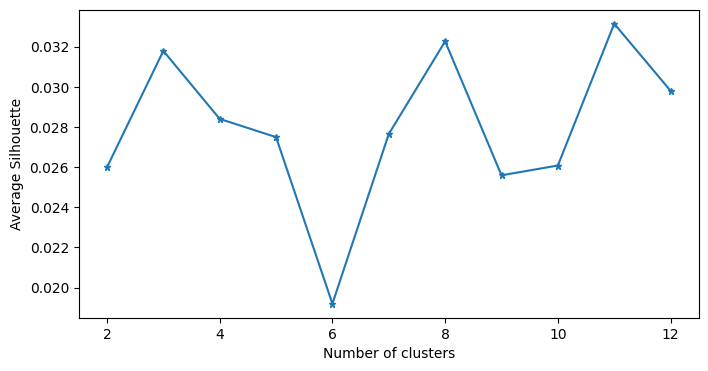
\includegraphics[scale=0.4]{../images/mnist_kmedoids_silhouette.png}
    \caption{Indice de silhouette en fonction du nombre de clusters}\label{fig:mnist_kmedoids_silhouette}
\end{figure}

D'après la figure \ref{fig:mnist_kmedoids_silhouette}, on remarque que \textbf{l'indice de silhouette est maximal pour 11 clusters}.
S'il s'agit du maximum de l'indice de silhouette en fonction de k, la valeur est de 0,331, ce qui n'est pas très proche de 1.
Cela peut signifier que la séparation entre les clusters n'est pas optimale.
Si l'on compare les indices de silhouette de K-means et K-medoids, on remarque qu'il est nettement plus aisé de choisir le nombre de clusters pour K-means.
En effet, pour K-means, l'indice de silhouette est maximal pour 7 clusters, pour une valeur d'environ 0,75, alors que pour K-medoids, il est maximal pour 11 clusters pour une valeur de 0,331.

\begin{figure}[h!]
    \centering
    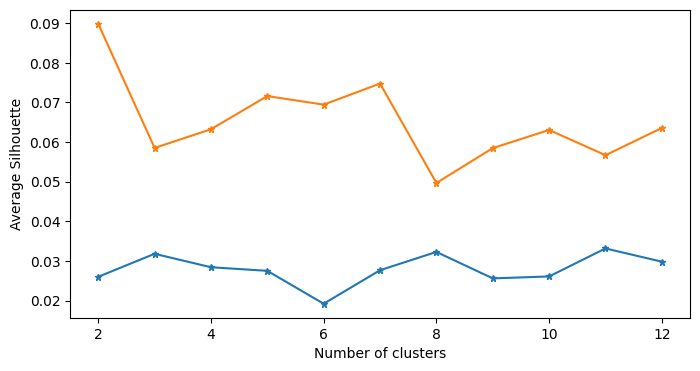
\includegraphics[scale=0.4]{../images/mnist_comparison_silhouette.png}
    \caption{Indice de silhouette en fonction du nombre de clusters pour K-means et K-medoides}\label{fig:mnist_comparison_silhouette}
\end{figure}

Nous gardons pour le moment 10 clusters.

\subsection{Étude des performances en fonction du nombre clusters : méthode alternative}

Ici, nous procédons à l'analyse de la matrice de confusion pour certains des nombres de clusters.


\paragraph{Matrice de confusion pour 10 clusters}
On peut aussi étudier la matrice de confusion pour chaque nombre de clusters.
Celle ci représente pour la ligne $i$ et la colonne $j$, le nombre de point de label $i$ qui sont dans le cluster $j$.

Dans ce paragraphe, nous comparerons les matrices de confusion dans le cas de 8, 10 et 11 clusters, valeurs maximales de l'indice de silhouette.

Pour le choix de 10 clusters, on obtient une matrice de taille 10x10.

\[
\begin{bmatrix}
368 & 38 & 6 & 6 & 13 & 43 & 3 & 5 & 9 & 510 \\
0 & 0 & 533 & 587 & 4 & 0 & 2 & 1 & 0 & 0 \\
3 & 11 & 388 & 143 & 11 & 126 & 59 & 27 & 108 & 115 \\
5 & 50 & 65 & 193 & 20 & 24 & 48 & 605 & 1 & 21 \\
6 & 85 & 149 & 44 & 309 & 27 & 334 & 2 & 20 & 4 \\
18 & 138 & 71 & 126 & 53 & 117 & 110 & 177 & 9 & 44 \\
32 & 197 & 31 & 47 & 4 & 182 & 2 & 0 & 506 & 13 \\
2 & 5 & 103 & 68 & 477 & 1 & 403 & 1 & 0 & 10 \\
5 & 99 & 215 & 141 & 16 & 13 & 176 & 249 & 15 & 15 \\
14 & 44 & 48 & 38 & 408 & 3 & 400 & 8 & 4 & 11 \\
\end{bmatrix}
\]
\captionof{table}{Matrice de confusion pour 10 clusters}

\paragraph{Analyse par colonne}
Chaque colonne représente un cluster.

En raisonnant de la même façon que pour K-means, on remarque que la première colonne est très hétérogène, 
ce qui signifie que dans ce cluster, le chiffre 0 est bien représenté avec 368 itérations, alors que le nombre 
de points des autres labels ne dépasse 32.
A l'inverse, la deuxième colonne possède une variance très faible, ce qui est cohérent en raison de son homogénéité.
Il est donc cohérent de dire que la première colonne relève d'un bon cluster, tandis que la deuxième non.

\paragraph{Analyse par ligne}
Chaque ligne représente un label.

De la même manière, on cherche une répartition hétérogène des valeurs pour chaque ligne.
Remarquons par exemple que le label 3 est bien représenté par le 8e cluster, tandis que le label 1 est bien représenté par les 3e et 4e clusters, 
ce qui peut mener à des confusions.
Les autres lignes (et donc labels) de la matrice de confusion dans le cas de 10 clusters sont plutôt homogènes, et donc difficiles à identifier.


\paragraph{Matrice de confusion pour 11 clusters}

\[
\begin{smallmatrix}
11 & 22 & 60 & 16 & 6 & 766 & 4 & 5 & 4 & 92 & 15 \\
2 & 509 & 9 & 1 & 16 & 0 & 0 & 1 & 589 & 0 & 0 \\
449 & 111 & 20 & 19 & 90 & 29 & 38 & 20 & 171 & 0 & 44 \\
138 & 104 & 324 & 82 & 11 & 31 & 28 & 10 & 60 & 239 & 5 \\
2 & 32 & 45 & 206 & 233 & 1 & 386 & 29 & 25 & 5 & 16 \\
1 & 110 & 255 & 58 & 128 & 22 & 61 & 5 & 35 & 177 & 11 \\
8 & 79 & 120 & 3 & 62 & 17 & 16 & 6 & 46 & 11 & 646 \\
0 & 72 & 46 & 63 & 63 & 1 & 161 & 600 & 59 & 3 & 2 \\
71 & 92 & 172 & 195 & 101 & 3 & 52 & 8 & 137 & 103 & 10 \\
0 & 24 & 21 & 374 & 79 & 11 & 387 & 50 & 15 & 15 & 2 \\
0 & 0 & 0 & 0 & 0 & 0 & 0 & 0 & 0 & 0 & 0 \\
\end{smallmatrix}
\]

\captionof{table}{Matrice de confusion pour 11 clusters}


En effectuant une analyse par colonnes, on peut voir qu'à priori les colonnes 1, 8, 10 et 11 sont relativement hétérogènes, et donc à priori les clusters sont de bonne qualité.
En procédant par ligne, nous remarquons que les labels ne sont pas particulièrement bien identifiés. Ceci paraît étonnant dans la mesure où à priori 11 clusters est le nombre optimal, et donc le résultat, montré par la matrice de confusion, devrait être meilleur que dans le cas de 10 clusters, ce qui n'est pas nécessairement le cas.


\paragraph{Matrice de confusion pour 8 clusters}

\[
\begin{bmatrix}
22 & 17 & 2 & 453 & 33 & 436 & 37 & 1 \\
3 & 6 & 1110 & 0 & 6 & 0 & 2 & 0 \\
65 & 45 & 369 & 1 & 8 & 33 & 49 & 421 \\
689 & 58 & 102 & 2 & 119 & 42 & 10 & 10 \\
7 & 523 & 87 & 0 & 4 & 7 & 350 & 2 \\
174 & 109 & 193 & 7 & 330 & 15 & 33 & 2 \\
11 & 178 & 260 & 48 & 117 & 263 & 115 & 22 \\
9 & 756 & 149 & 0 & 2 & 22 & 131 & 1 \\
236 & 247 & 279 & 3 & 116 & 26 & 23 & 14 \\
34 & 688 & 54 & 3 & 18 & 3 & 176 & 2 \\
\end{bmatrix}
\]
\captionof{table}{Matrice de confusion pour 8 clusters}

Les colonnes 4 et 8 sont très hétérogènes et donc témoignent de la qualité des deux clusters y correspondant.
Le label 1 est également extrêmement bien identifié. Le label 9, lui aussi, est très bien représenté.
Le reste des colonnes et lignes sont relativement homogènes.


\subsection{Comparaison de la précision du clustering}

\begin{figure}[h!]
    \centering
    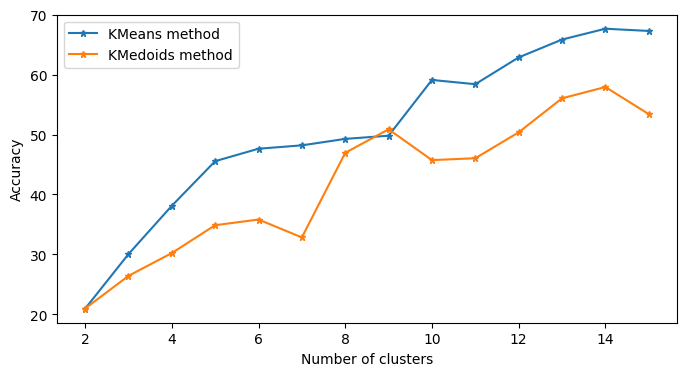
\includegraphics[scale=0.4]{../images/mnist_comparison_accuracy.png}
    \caption{Précision du clustering en fonction du nombre de clusters pour K-means et K-medoides}\label{fig:mnist_comparison_accuracy}
\end{figure}

D'après la figure \ref{fig:mnist_comparison_accuracy}, nous remarquons que la précision du clustering avec la méthode K-means croît plus vite que K-medoïdes. Il semble aussi que la précision du clustering avec K-medoïdes converge vers un pourcentage plus bas que K-means. Néanmoins, on peut remarquer que dans les deux cas, à partir de 8 clusters, \textbf{la précision du clustering avec ces méthodes avoisine voire dépasse les 50\%} ce qui atteste de la qualité de ces méthodes dans notre cas.

\subsection{Comparaison du temps de calcul des deux algorithmes K-means et K-medoids}

Nous avons comparé le temps de calcul des deux algorithmes K-means et K-medoids pour la base de données MNIST, à l'aide de la librairie Time.

Dans le cas de K-means, la mise en place de l'algorithme ainsi que l'apprentissage non supervisé prend 0,563 secondes à se faire. Dans le cas de K-Medoids, les mêmes opérations prennent 3,890 secondes à se faire.

Ce résultat était attendu étant donné que si K-médoïdes est censé être plus robuste à priori aux valeurs absurdes, il est plus coûteux en calcul et donc prend plus de temps à tourner.


\section{Étude du Modèle à Mélange de Gaussiennes}
\subsection{Présentation du modèle}
Pour cette étude, nous travaillons sur un set de données "isotropic Gaussian blobs for clustering". Ceci signifie que les points de données sont générés suivent une distribution gaussienne isotropique, comme montré en figure \ref{fig:gmm_generate_data}.

\begin{figure}[h!]
    \centering
    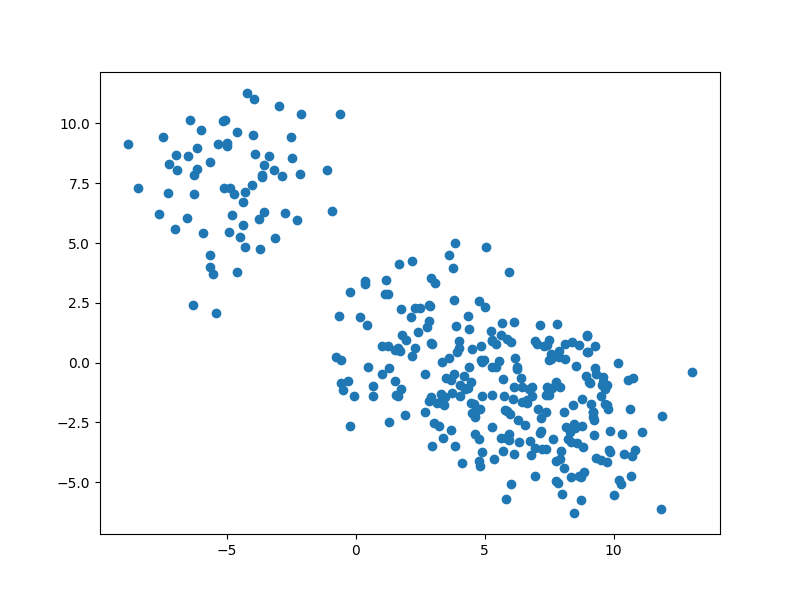
\includegraphics[scale=0.4]{../images/gmm_generate_data.png}
    \caption{}\label{fig:gmm_generate_data}
\end{figure}

5 centres ont été choisis dans notre cas, et se retrouveront donc centres de chacun des 5 clusters déterminés par une distribution gaussienne. Ceux-ci sont repérables en rouge sur la figure \ref{fig:gmm_centers}

\begin{figure}[h!]
    \centering
    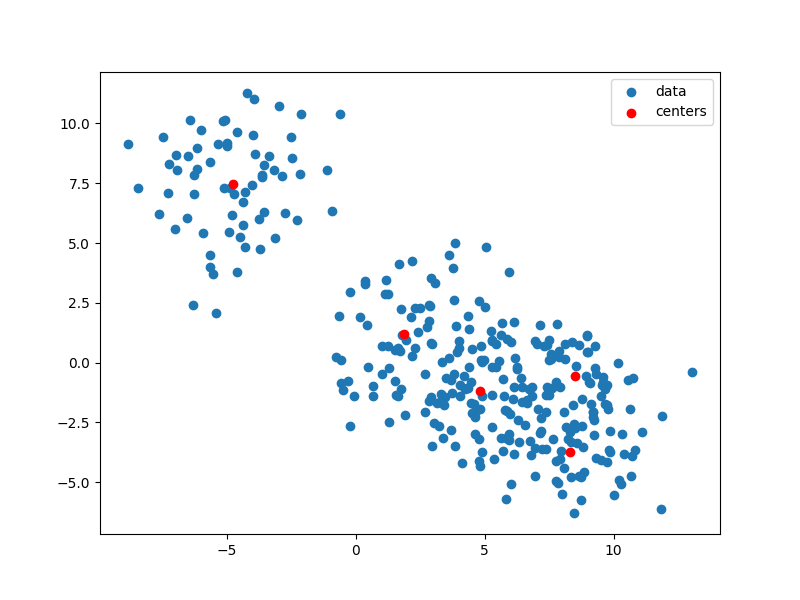
\includegraphics[scale=0.4]{../images/gmm_centers.png}
    \caption{}\label{fig:gmm_centers}
\end{figure}

Nous pouvons repérer chaque cluster et ses centres, comme affiché en figure \ref{fig:gmm_clusters_centers}

\begin{figure}[h!]
    \centering
    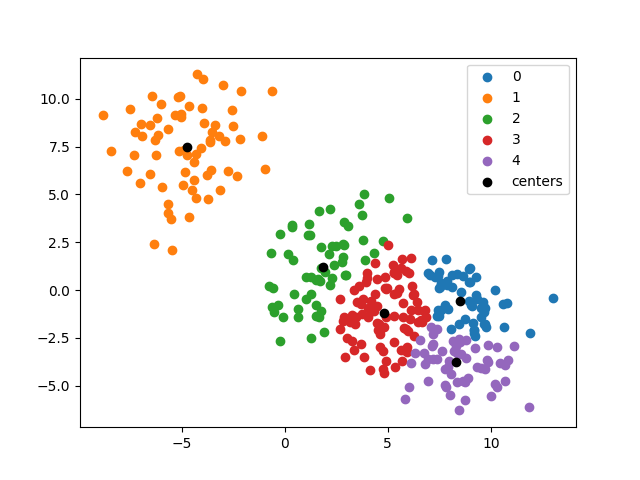
\includegraphics[scale=0.4]{../images/gmm_clusters_centers.png}
    \caption{}\label{fig:gmm_clusters_centers}
\end{figure}

\subsection{Analyse du clustering par GMM avec Calinski-Harabasz}

Le score de Calinski-Harabasz peut être une solution pour trouver le nombre optimal de clusters.

La figure \ref{fig:gmm_ch_score} permet de déterminer le nombre optimal de clusters pour la méthode du modèle à mélange de gaussiennes.
Le score de Calinski-Harabasz doit se trouver dans une plage de 0 à l'infini, 0 correspondant à une mauvaise classification.

\begin{figure}[h!]
    \centering
    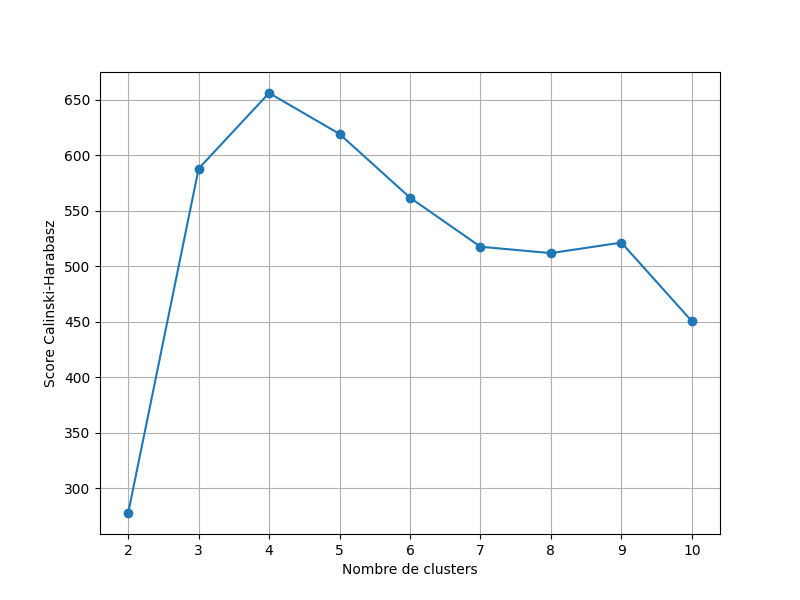
\includegraphics[scale=0.4]{../images/calinski_harabasz_scores_gmm.png}
    \caption{}\label{fig:gmm_ch_score}
\end{figure}

Nous cherchons à garder le nombre de clusters correspondant à un score maximal. En l'occurence, \textbf{le nombre optimal de clusters est de 4}.

\section{Limitations de KMeans: DBSCAN}

On a vu que l'algorithme KMeans n'était pas très performant pour la base de données MNIST.
De plus, clusterisé sous forme de cercle n'est pas toujours adapté pour des données de forme complexe.
On va donc le comparer à l'algorithme DBSCAN pour un ensemble de données représentant en forme de lune.

\begin{figure}[h!]
    \centering
    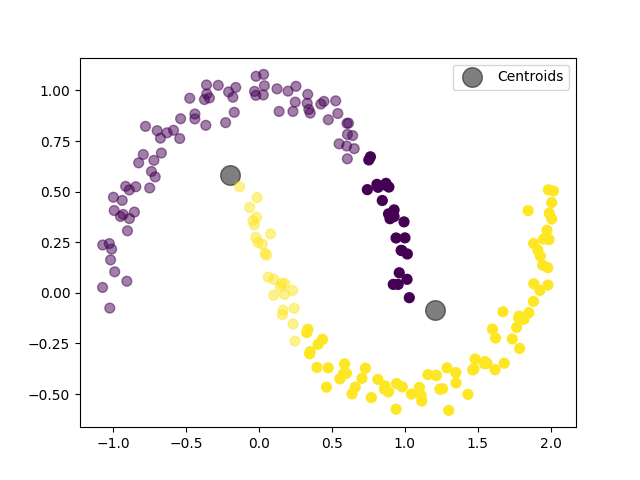
\includegraphics[scale=0.5]{../images/moon_dbscan.png}
    \caption{Résultat des clusterings par KMeans et DBSCAN}\label{fig:dbscan_moon}
\end{figure}

Ici on repère la clusterisation faite par KMeans en fonction de la transparence des points et par la couleur pour DBSCAN. 
On remarque ici que les clusters obtenus sont très différents. 
KMeans clusterise en forme de cercle tandis que DBSCAN clusterise par proximité et arrive à bien distinguer les deux lunes.

\section{KMeans pour la segmentation d'images}

On va maintenant utiliser l'algorithme KMeans pour segmenter une image en 3 couleurs,
c'est à dire qu'on va chercher à regrouper les pixels de l'image en 3 clusters.
Cela va nous permettre de réduire le nombre de couleurs de l'image.

Pour cela on va travailler sur une image de chien sur laquelle on va clusteriser
les pixels en 2.
\begin{figure}[h!]
    \centering
    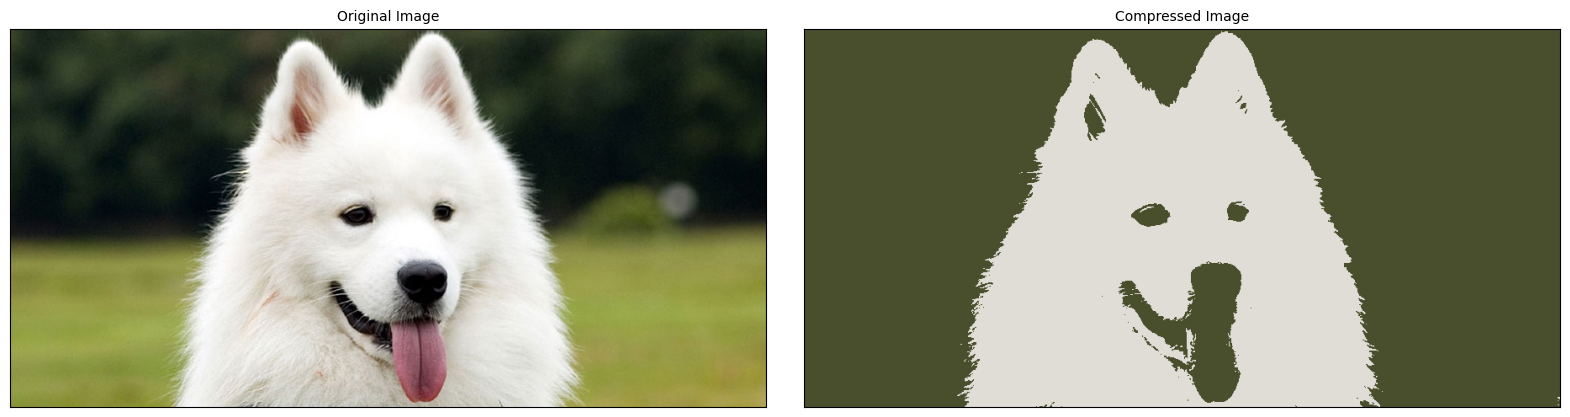
\includegraphics[scale=0.2]{../images/dog_compressed.png}
    \caption{Image de chien}\label{fig:dog}
\end{figure}


KMeans a bien réussi à segmenter l'image en deux couleurs. On distingue encore clairement le chien du fond.

On réitère l'opération pour différents nombres de clusters.

\begin{figure}[h!]
    \centering
    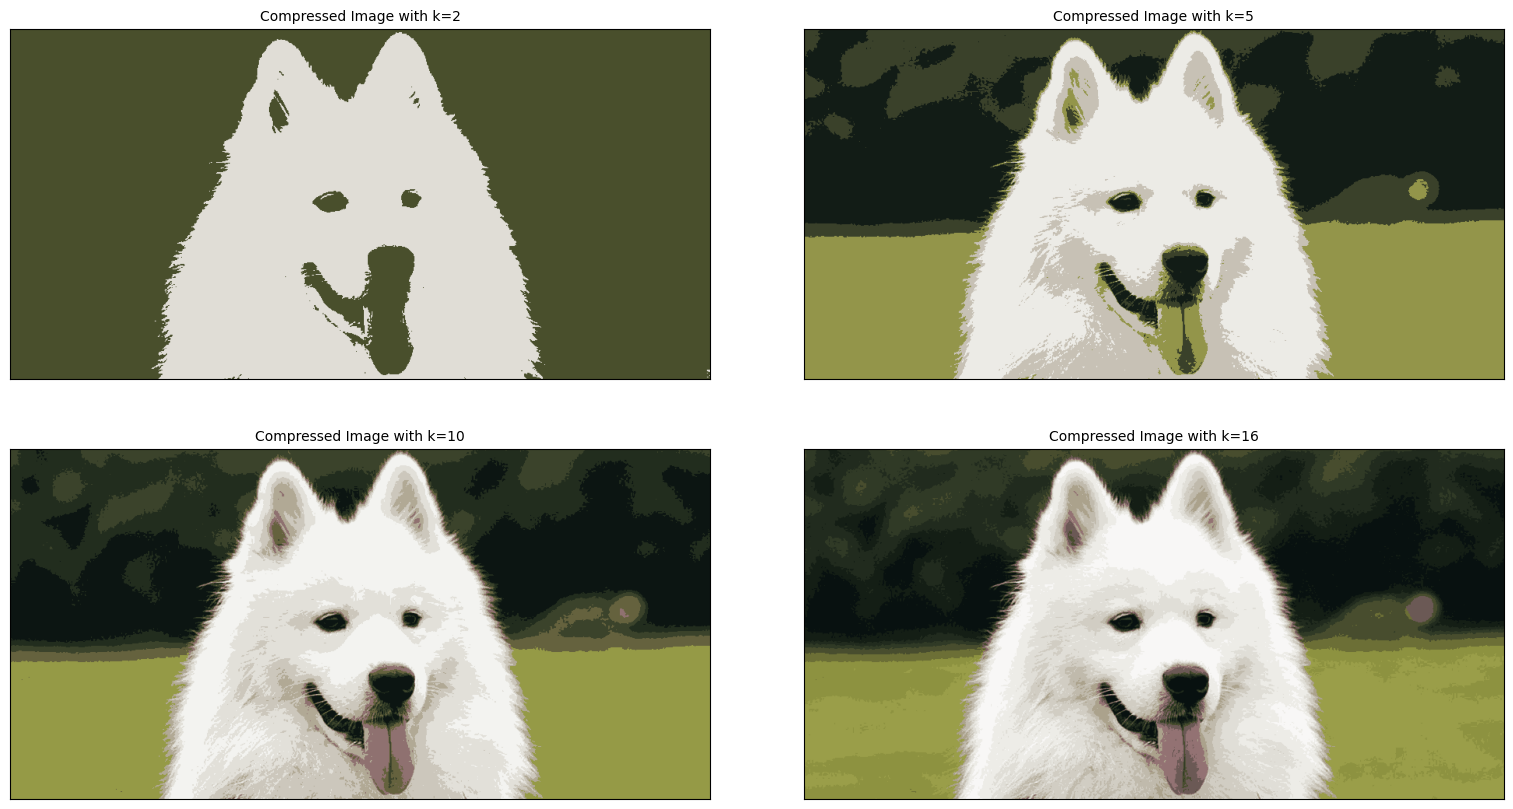
\includegraphics[scale=0.2]{../images/dog_segmented_comparaison.png}
    \caption{Segmentation pour différent nombre de clusters}\label{fig:dog_kmeans}
\end{figure}

On remarque que l'image devient de plus en plus nette avec l'augmentation du nombre de clusters.
Cela est cohérent car on cherche à réduire le nombre de couleurs de l'image.
On a donc pu voir que l'algorithme KMeans est bien adapté pour la segmentation d'images.

\section{Conclusion}

On a étudié les performances de l'algorithme KMeans et KMédoids sur la base de données MNIST 
à travers différentes métriques: la matrice de confusion, la variance normalisée par colonne, l'entropie et le taux de bon fonctionnement.
Ces métriques ont permis de noter les performances de l'algorithme pour différents nombres de clusters.
Nous avons également pu analyser le modèle à mélange de gaussiennes pour un set de données généré suivant une distribution gaussienne isotropique.
Enfin, nous avons comparé les performances de KMeans et DBSCAN pour le clustering de données de forme complexe, et nous avons utilisé KMeans pour la segmentation d'images.

En somme, nous avons pu voir que KMeans est un algorithme performant pour la segmentation d'images, mais qu'il n'est pas adapté pour des données de forme complexe.

\end{document}